\documentclass[12pt,letterpaper]{article}
\usepackage[top=0.85in,left=1in,footskip=0.75in,marginparwidth=2in]{geometry}

% use Unicode characters - try changing the option if you run into troubles with special characters (e.g. umlauts)
\usepackage[utf8]{inputenc}

% clean citations
\usepackage{cite}

% hyperref makes references clicky. use \url{www.example.com} or \href{www.example.com}{description} to add a clicky url
\usepackage{nameref,hyperref}

% line numbers
\usepackage[right]{lineno}

% improves typesetting in LaTeX
\usepackage{microtype}
\DisableLigatures[f]{encoding = *, family = * }

% text layout - change as needed
\raggedright
\setlength{\parindent}{0.5cm}
\textwidth 6.5in 
\textheight 9in
\renewcommand{\baselinestretch}{1.5}

% use adjustwidth environment to exceed text width (see examples in text)
\usepackage{changepage}

% adjust caption style
\usepackage[aboveskip=1pt,labelfont=bf,labelsep=period,singlelinecheck=off]{caption}

% remove brackets from references
\makeatletter
\renewcommand{\@biblabel}[1]{\quad#1.}
\makeatother

% headrule, footrule and page numbers
\usepackage{lastpage,fancyhdr,graphicx}
\usepackage{epstopdf}
\pagestyle{myheadings}
\pagestyle{fancy}
\fancyhf{}
\rfoot{\thepage/\pageref{LastPage}}
\renewcommand{\footrule}{\hrule height 2pt \vspace{2mm}}
\fancyheadoffset[L]{2.25in}
\fancyfootoffset[L]{2.25in}

% use \textcolor{color}{text} for colored text (e.g. highlight to-do areas)
\usepackage{color}

% define custom colors (this one is for figure captions)
\definecolor{Gray}{gray}{.25}

% this is required to include graphics
\usepackage{graphicx}
\graphicspath{{../figures/}}

% use if you want to put caption to the side of the figure - see example in text
\usepackage{sidecap}

% use for have text wrap around figures
\usepackage{wrapfig}
\usepackage[pscoord]{eso-pic}
\usepackage[fulladjust]{marginnote}
\reversemarginpar

% document begins here
\begin{document}
\vspace*{0.35in}

% title goes here:
\begin{flushleft}
{\Large
\textbf\newline{Are essential genes conserved?}
}
\newline
% authors go here:
\\
%Fatemeh Ashari Ghomi\textsuperscript{1},
%Paul P. Gardner\textsuperscript{1,*},
%Lars Barquist\textsuperscript{2}
%\\
%\bigskip
%\bf{1} University of Canterbury
%\\
%\bf{2} Wurzburg University
%\\
%\bigskip
%* paul.gardner@canterbury.ac.nz

\end{flushleft}

\section*{Abstract}
%Fitting multiple figures into very tight manuscripts while keeping it pleasant to read is challenging. Therefore figures are often simply attached to the very end of a manuscript file. While easier for the authors, this practice is inconvenient for readers. This \LaTeX template shows how to generate a compiled PDF with figures embedded into the text. It provides several examples of how to embed figures or tables directly into the text thus giving you a range of options from which you should choose the one best suited for your manuscript. Check out Schlegel et al., (2016) as example of use \cite{Schlegel2016}.
%
% now start line numbers
%\linenumbers

% the * after section prevents numbering
\section*{Introduction}
Studying the essentiality of genes helps with identifying the fundamental processes necessary for cell viability \cite{juhas_essence_2011}. So far, scientists have studied the essential genes in organisms from different domains of life \cite{luo_deg_2014}. The results have led to new insights for developing new antibiotics that target essential genes of pathogenic bacteria \cite{clatworthy_targeting_2007, peters_comprehensive_2016} and synthesising new genomes \cite{hutchison_global_1999, hutchison_design_2016}. Researchers have used different methods for studying the essentility of genes in prokaryotes. Baba et al.\@ \cite{baba_construction_2006} have made a library of single gene deletions using phage lambda Red recombination system to screen essential genes while another group have used antisense RNA knockdowns for this purpose \cite{xu_staphylococcus_2010}. Another method that is widely used due to its simplicity and accuracy is transposon mutagenesis along with high-throughput sequencing \cite{gawronski_tracking_2009, van_opijnen_tn-seq:_2009, langridge_simultaneous_2009, christen_essential_2011, goodman_identifying_2011, wetmore_rapid_2015, rubin_essential_2015}. In this method, pools of single insertion mutants are constructed using transposon mutagenesis and the effect of each mutation on the survival of mutants is evaluated by sequencing the survivors \cite{barquist_approaches_2013}. This can lead to the identification of essential genes.

Although the essentiality of genes has been studied in a variety of organisms, there is still room to study the evolutionary conservation of essentiality. Curtis and Brun \cite{curtis_identification_2014} have studied the essentiality changes in cell cycle genes of three alpha-proteobacteria strains: \textit{Caulobacter crescentus}, \textit{Brevundimonas subvibrioides}, and \textit{Agrobacterium tumefaciens}. Canals et al.\@ \cite{canals_high-throughput_2012} have compared the essentiality of genes in \textit{Salmonella} typhimurium and \textit{Salmonella} Typhi. In a similar study, Barquist et al.\@ \cite{barquist_comparison_2013} have used transposon-directed insertion-site sequencing to study the differentiation of the essentiality of genes in \textit{Salmonella} serovars Typhi and Typhimurium which has led to divergence in their pathogenecity and host ranges. We extend this research by studying 13 bacterial strains from Enterobacteriaceae. These strains and \textit{Escherichia coli} K-12 MG1655 studied by Baba et al.\@ \cite{baba_construction_2006} are depicted in Fig.\@ \ref{fig:species-tree}.

\begin{figure}
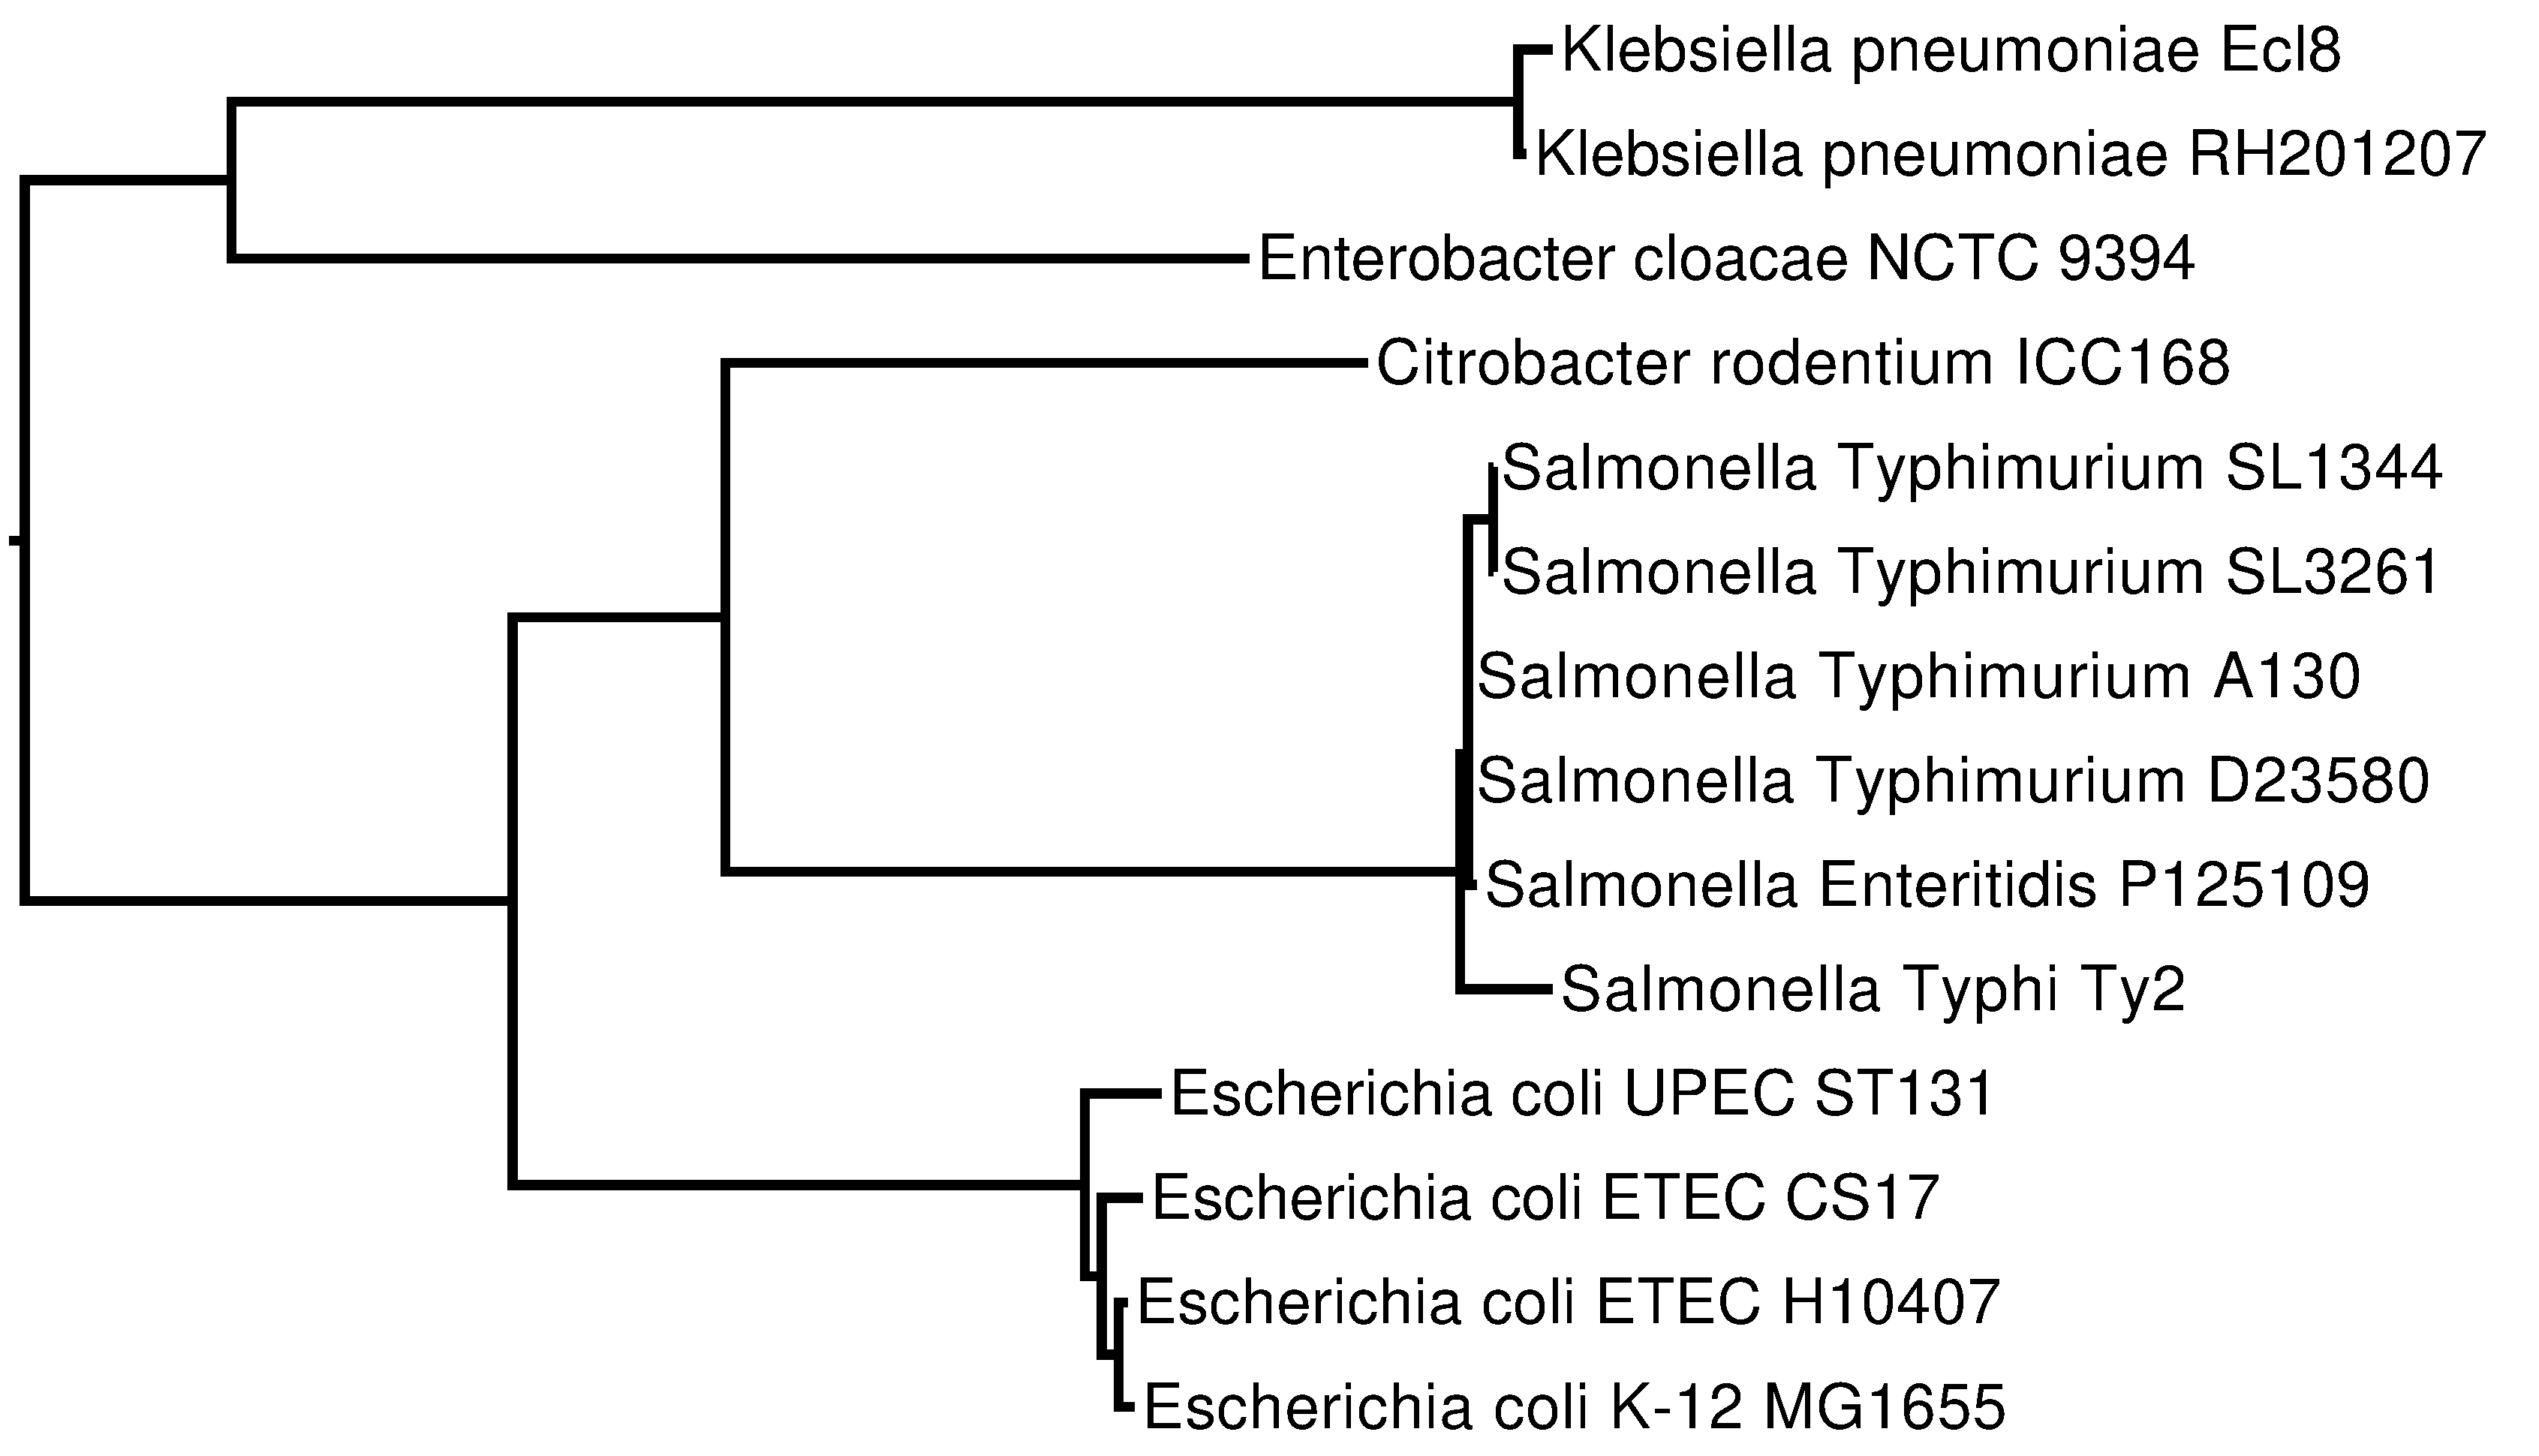
\includegraphics[scale=0.2]{phylosift-aa-raxmlbootstrap.pdf}
\caption{The species tree containing the 13 strains under study and Escherichia \textit{coli} K-12 MG1655 studied in Keio collection \cite{baba_construction_2006}. We have generated the tree by running RAxML \cite{stamatakis_raxml_2014} on Phylosift \cite{darling_phylosift:_2014} amino acid markers.}
\label{fig:species-tree}
\end{figure}

\textcolor{red}{\{A summary of what we have done\}}

\section{Transposon mutagenesis}
During evolution species can gain or lose genes. We have investigated if these gene gain and losses are related to the essentiality of the genes themselves. For this, we have evaluated the essentiality of genes and their conservation and the relationship between these two. We have studied 2 \textit{Klebsiella} strains, an \textit{Enterobacter} strain, a \textit{Citrobacter} strain, 6 \textit{Salmonella} strains, and 3 \textit{Escherichia} strains and compared the essentiality of genes in these strains and \textit{Escherichia coli} K-12 MG1655 from another study \cite{baba_construction_2006}. These strains are all selected from Enterobacteriaceae family. Enterobacteriaceae is a well characterised family of Gram-negative bacteria with a variety of host ranges and pathogenecity \cite{brenner_bergeys_2006}. Here, we perform a transposon-directed insertion-site sequencing experiment to study the conservation of essentiality of genes in strains from 5 different species in this family.

Transposon mutagenesis is frequently used for the study of essentiality. We have used Tn5 transposon to generate single inserted mutants and placed our mutants in a selective media for Tn5. We have picked the mutants and pooled them and performed PCR enrichment using the method described in \cite{barquist_tradis_2016}. Then, we have sequenced the fragments and mapped them back to the genome to figure out the number of insertions that have been tolerated in each position of the genome. The number of insertions in a gene implies the degree of essentiality for that gene.

%\subsection{Essentiality}
We have used a value called insertion index to evaluate the essentiality of a gene. This value is calculated by summing up the number of transposon insertion sites observed in a gene. Since the lengths of the genes are different, we have normalised the insertion index by dividing it by gene length. Our experiment has been performed on different strains and the library density is different in each experiment. Therefore, in order to make the insertion indices comparable in all the strains, we have normalised our insertion indices by the ratio between the number of insertions in the whole genome and the length of the genome. We have not studied genes shorter than 100 base-pairs as they might not be targeted by any transposon due to their shortness. 

We have divided the genes into three groups: essential genes, ambiguous, non-essential genes, and beneficial losses. We have utilised the pipeline introduced by Barquist et al.\@ \cite{barquist_tradis_2016} to evaluate the essentiality of genes. The insertion index distribution plot has two peaks and a heavy tail as shown in Fig.\@ \ref{fig:iidist-species}. The first peak shows the genes with no or just a few insertions which are considered as essential genes. We have fitted an exponential distribution to the first peak and a gamma distribution to the second one. Then, we have calculated the log odds ratio for belonging to each of these distributions for each gene. The region that has log odds value between -2 and 2 is called the ambiguous region, the genes belonging to the first peak are essential and the rest of the genes are not essential. Among genes that are not essential, any gene for which the value of the cumulative distribution function for the gamma distribution is greater than or equal to 0.99 is considered as a beneficial loss and the other genes are non-essential genes.

\begin{figure*}
\centering
\begin{tabular}{c c c}
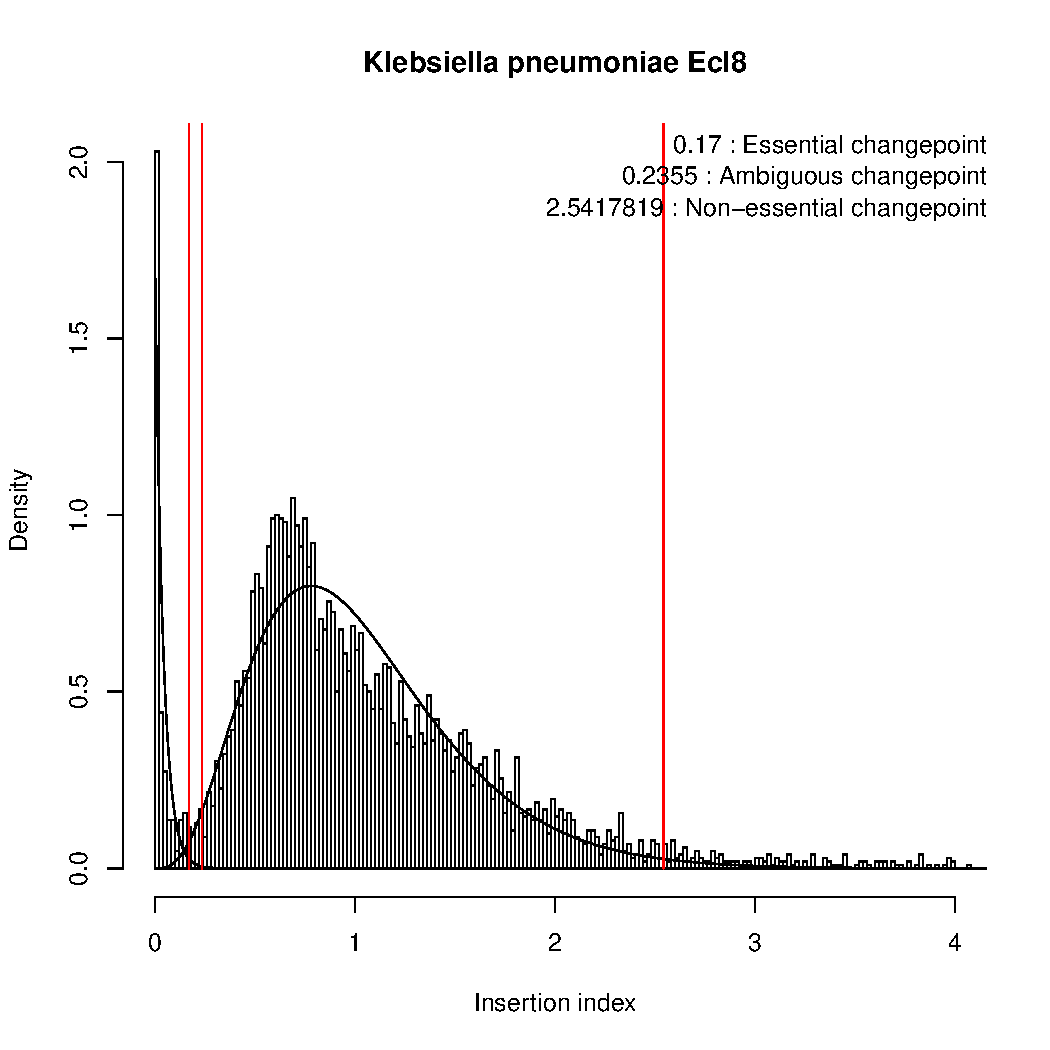
\includegraphics[page=1, scale=0.25]{essentiality.pdf}&
\includegraphics[page=2, scale=0.25]{essentiality.pdf}&
\includegraphics[page=3, scale=0.25]{essentiality.pdf}\\
\includegraphics[page=4, scale=0.25]{essentiality.pdf}&
\includegraphics[page=5, scale=0.25]{essentiality.pdf}&
\includegraphics[page=6, scale=0.25]{essentiality.pdf}\\
\includegraphics[page=7, scale=0.25]{essentiality.pdf}&
\includegraphics[page=8, scale=0.25]{essentiality.pdf}&
\includegraphics[page=9, scale=0.25]{essentiality.pdf}\\
\includegraphics[page=10, scale=0.25]{essentiality.pdf}&
\includegraphics[page=11, scale=0.25]{essentiality.pdf}&
\includegraphics[page=12, scale=0.25]{essentiality.pdf}\\
&\includegraphics[page=13, scale=0.25]{essentiality.pdf}&\\
\end{tabular}
\caption{Plots show the insertion index distribution for each genome. The plots are divided into 4 regions using red lines. These regions from left to right are: essential, ambiguous, non-essential, and beneficial loss.}
\label{fig:iidist-species}
\end{figure*}

%\section{Are transposons biased towards certain positions?}
\section{Are there biases in transposon mutagenesis data?}
To evaluate the essentiality of a gene, we use the number of insertions within that gene. However, if the transposons are biased to specific regions in the genome, it results in false predictions and influences the accuracy of our analysis. Different articles have reported biases in transposon mutagenesis \cite{barquist_comparison_2013, rubin_essential_2015, kimura_nucleoid_2016}. We have performed a detailed study of these biases. The biases that we have studied include: gene length bias, origin of replication bias, preferred insertion motif bias, and positional bias within genes.

\subsection{Length bias}
Short genes are less probable to be hit by transposons and so the genes that are very short might have no insertions. As a result, normalising the number of insertions by the length of the genes does not affect the essentiality level of these genes. 
In Fig.\@ \ref{fig:length-bias} we have studied if the length of genes can influence their essentiality and we have found no correlation between length and insertion index. It seems that the insertion density in our experiment is high enough to make it possible for every gene to be hit by transposons.
\begin{figure*}
\centering
\includegraphics[page=42, scale=0.3]{biases.pdf}
\caption{The plot shows the lengths of the genes against their insertion indices. The red line shows the loess curve when the smoothness parameter is $0.2$.}
\label{fig:length-bias}
\end{figure*}

\subsection{Origin of replication bias}
To study the bias towards the position of the genes, we plotted the insertion index for each gene versus the distance of the gene from the origin of replication normalised by the length of the genome. Fig.\@ \ref{fig:distance-bias} shows the results. The red line is a loess curve that has been fitted to the data when the smoothness parameter equals $0.2$. The figure indicates that the insertion indices decrease when the genes are located further from the origin of replication. A possible explanation for this phenomenon is that the bacteria were under replication while being infected with transposons. Therefore, the number of gene copies close to the origin of replication was greater and more insertions have occurred in these genes. To overcome this bias, we have normalised our insertion indices by dividing the value of the insertion index by the predicted value by loess for that position and then multiplying this value by the average insertion index.

{\bf mention possible confounding factor for this study. Essential genes may (are???) non-uniformly distributed in the genome (I presume they are clustered near the origin). This would be expected to lower the insertion index near the origin, however, the number of non-essential genes is $\approx 10\times$ the number of essential genes, therefore the signature of biased numbers of insertions near the origin remains. }

\begin{figure*}
\centering
\begin{tabular}{c c c}
\includegraphics[page=2, scale=0.25]{biases.pdf}&
\includegraphics[page=5, scale=0.25]{biases.pdf}&
\includegraphics[page=8, scale=0.25]{biases.pdf}\\
\includegraphics[page=11, scale=0.25]{biases.pdf}&
\includegraphics[page=14, scale=0.25]{biases.pdf}&
\includegraphics[page=17, scale=0.25]{biases.pdf}\\
\includegraphics[page=20, scale=0.25]{biases.pdf}&
\includegraphics[page=23, scale=0.25]{biases.pdf}&
\includegraphics[page=26, scale=0.25]{biases.pdf}\\
\includegraphics[page=29, scale=0.25]{biases.pdf}&
\includegraphics[page=32, scale=0.25]{biases.pdf}&
\includegraphics[page=35, scale=0.25]{biases.pdf}\\
&\includegraphics[page=38, scale=0.25]{biases.pdf}&\\
\end{tabular}
\caption{The plots show the distance of the genes from DnaA gene normalised by the lengths of the genomes versus the insertion indices of the genes. The distance from DnaA gene has been calculated in both directions and then the minimum value has been used for distance. The red curves show the loess curve when the smoothness parameter is $0.2$.}
\label{fig:distance-bias}
\end{figure*}

{\bf PREFERRED INSERTION MOTIF BIAS:} We have tested whether our transposons are biased towards certain motifs. For this, we have generated a logo from 10 nucleotides flanking the 100 top most frequent insertion sites in each genome. The results are depicted in Fig.\@  \ref{fig:logos}. The results show a slight bias towards certain combinations of bases. In addition, we have investigated if the G-C content of genes can change the number of insertions by plotting the number of G-C bases in a gene normalised by the length of the gene versus insertion index Fig.\@  \ref{fig:GC-bias}. The red lines show the loess curve when the smoothness parameter is $0.2$. As the figure shows, when G-C content is less than $40\%$, the insertion index is low, however when it is higher than $50\%$, the insertion index is almost constant. A possible reason for this phenomena is the association of A-T rich sequences and histone-like nucleotide structuring (H-NS) proteins, which causes a reduction in the insertions in A-T rich regions \cite{kimura_nucleoid_2016}. The other reason is that the genes with low G-C content are enriched in mobile genetic elements compared to the genes with average G-C content (\ref{fig:gc-pval}) and this has caused seeing a different pattern of essentiality in that region.

\begin{itemize}
\item model H-NS binding sites? CGWTWHWww Lang et al (2007)
\item seems unlikely -- show bulk of genes are around 50\% G+C (add box-whisker plots to scatter diagrams?)
\item check Freed, Silander paper -- the missing piece of genome, was this low G+C? 
\end{itemize}

\begin{figure*}
\begin{tabular}{c c}
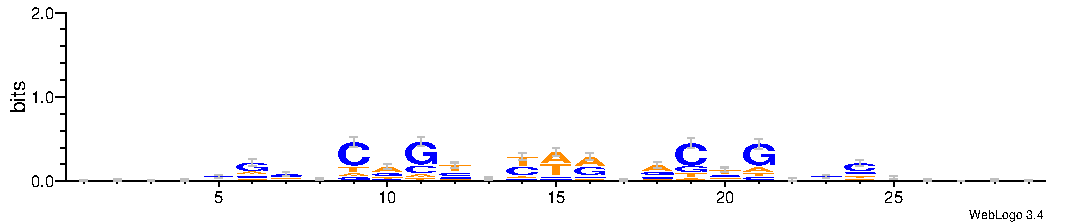
\includegraphics[scale=0.55]{100logo-bits.pdf}&
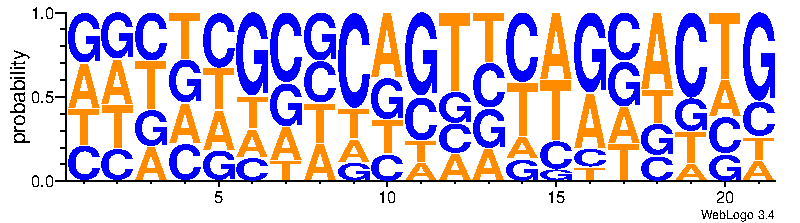
\includegraphics[scale=0.55]{100logo-prob.pdf}
\end{tabular}
\caption{We have generated sequence logo plots using sequences from 10 nucleotides flanking the 100 top most frequent insertion sites from each genome. On the left the height of each character corresponds to a bit score for that character (i.e. $2-\sum f_a\times\log_2f_a-\frac{1}{\ln2}\times\frac{3}{2\times n}$, where $f_a$ is the relative frequency of base $a$ and $n$ is the number of sequences). To put it in simple words, the height of the set of characters shows how biased that position is and the height of each character shows the amount of bias towards that character. On the right the height of each character shows the relative frequency of that character.}
\label{fig:logos}
\end{figure*}

\begin{figure*}
\centering
\begin{tabular}{c c c}
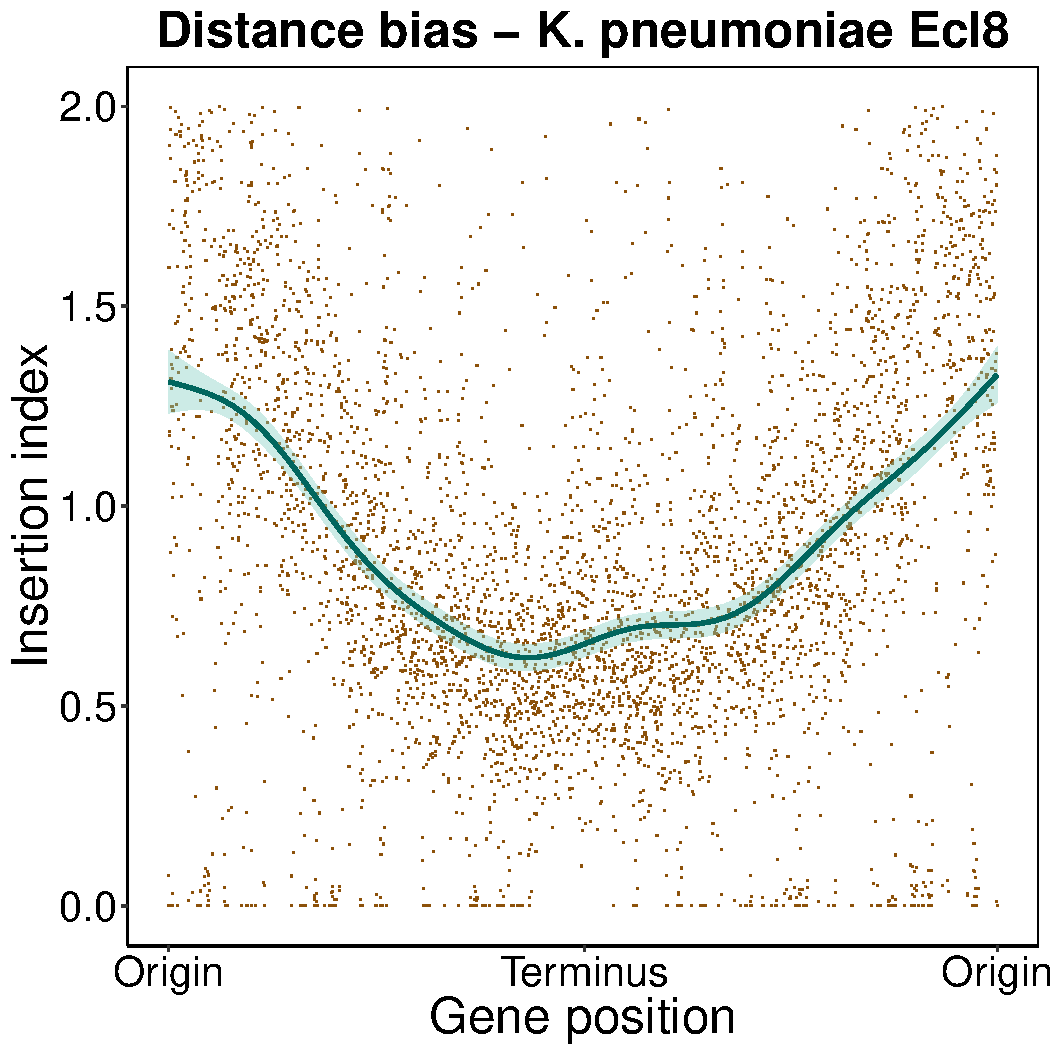
\includegraphics[page=1, scale=0.25]{biases.pdf}&
\includegraphics[page=4, scale=0.25]{biases.pdf}&
\includegraphics[page=7, scale=0.25]{biases.pdf}\\
\includegraphics[page=10, scale=0.25]{biases.pdf}&
\includegraphics[page=13, scale=0.25]{biases.pdf}&
\includegraphics[page=16, scale=0.25]{biases.pdf}\\
\includegraphics[page=19, scale=0.25]{biases.pdf}&
\includegraphics[page=22, scale=0.25]{biases.pdf}&
\includegraphics[page=25, scale=0.25]{biases.pdf}\\
\includegraphics[page=28, scale=0.25]{biases.pdf}&
\includegraphics[page=31, scale=0.25]{biases.pdf}&
\includegraphics[page=34, scale=0.25]{biases.pdf}\\
\includegraphics[page=37, scale=0.25]{biases.pdf}&&
\includegraphics[page=40, scale=0.25]{biases.pdf}\\
\end{tabular}
\caption{The plots show the ratio of G-C bases in the genes normalised by the lengths of the genes against their insertion indices. The red curves show the loess curve when the smoothness parameter is $0.2$.}
\label{fig:GC-bias}
\end{figure*}

\begin{figure*}
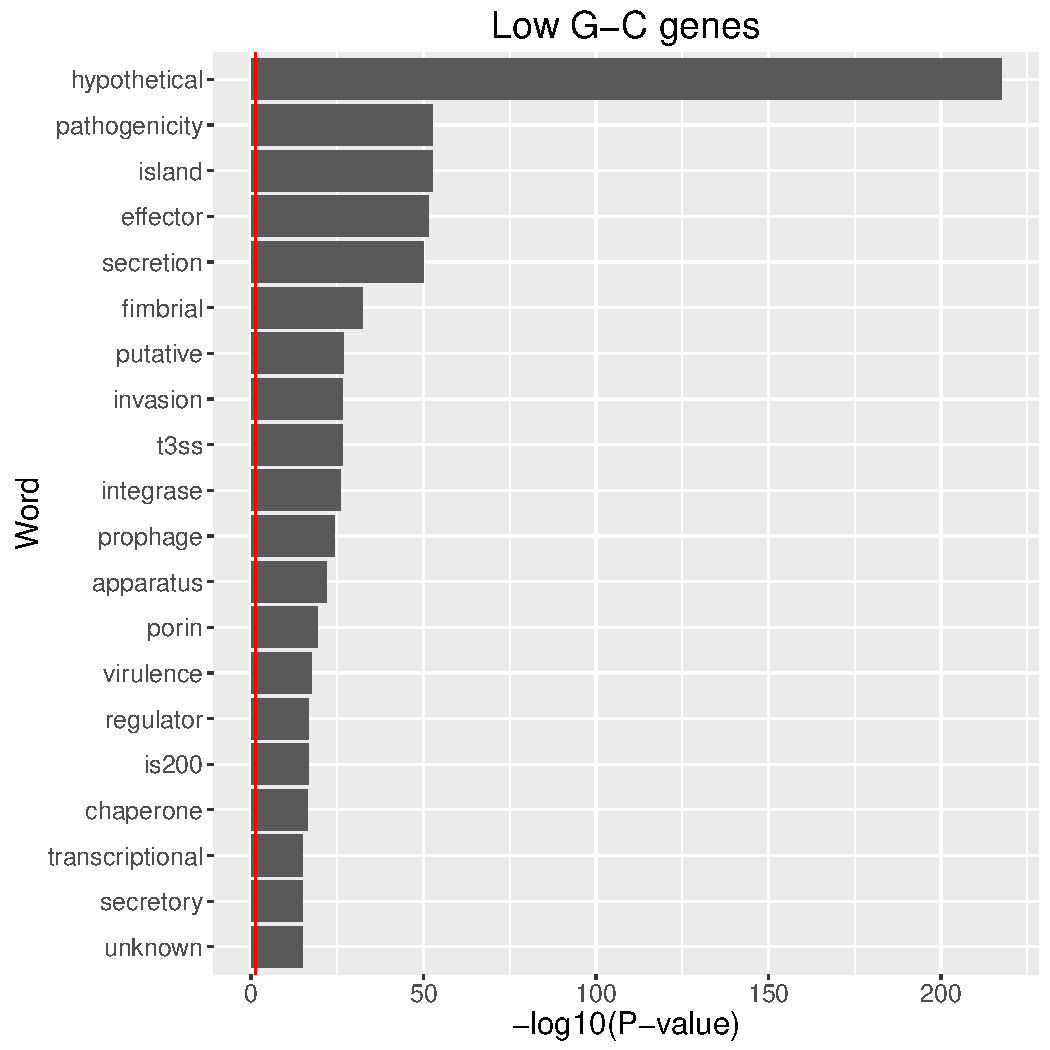
\includegraphics[scale=0.55]{lowgc-pval.pdf}
\caption{Word enrichment analysis for low G-C genes compared to genes with interquartile G-C level. The red line shows P-value = 0.05. The P-values have been calculated using Fisher's exact test and corrected using Benjamini-Hochberg-Yekutieli.}
\label{fig:gc-pval}
\end{figure*}

The other bias that we have considered is the bias towards certain locations in a gene. We have divided every gene into 100 bins and calculated the mean insertion index for each bin. Fig.\@ \ref{fig:insertion-position-bias} shows almost no bias towards any location. We have also studied the bias in each of the groups: essential genes, non-essential genes, and beneficial losses. The results imply that the number of insertions in the internal region of the essential genes is outnumbered by the number of insertions in the 5' and 3' ends while it is the opposite in beneficial losses. The case for the non-essential genes is similar to the average (Fig.\@ \ref{fig:insertion-position-bias}). High number of insertions at the 3' end of essential genes implies that the functional part of the genes are located before the insertions. On the other hand, high number of insertions at the 5' end of the essential genes indicates there might be alternative start codons in the 5' end or it might be because of alignment errors. \textcolor{red}{\{To be tested\}} We have calculated the insertion index for genes by ignoring $5\%$ from the 5' end and $20\%$ from the 3' end of the genes to overcome these biases. The insertion index distribution for each genome after correcting for all distance from the origin of replication bias and bias towards the position of insertion within genes is depicted in Fig.\@ \ref{fig:iidist-species-normalised}.

\begin{figure*}
\begin{tabular}{c c}
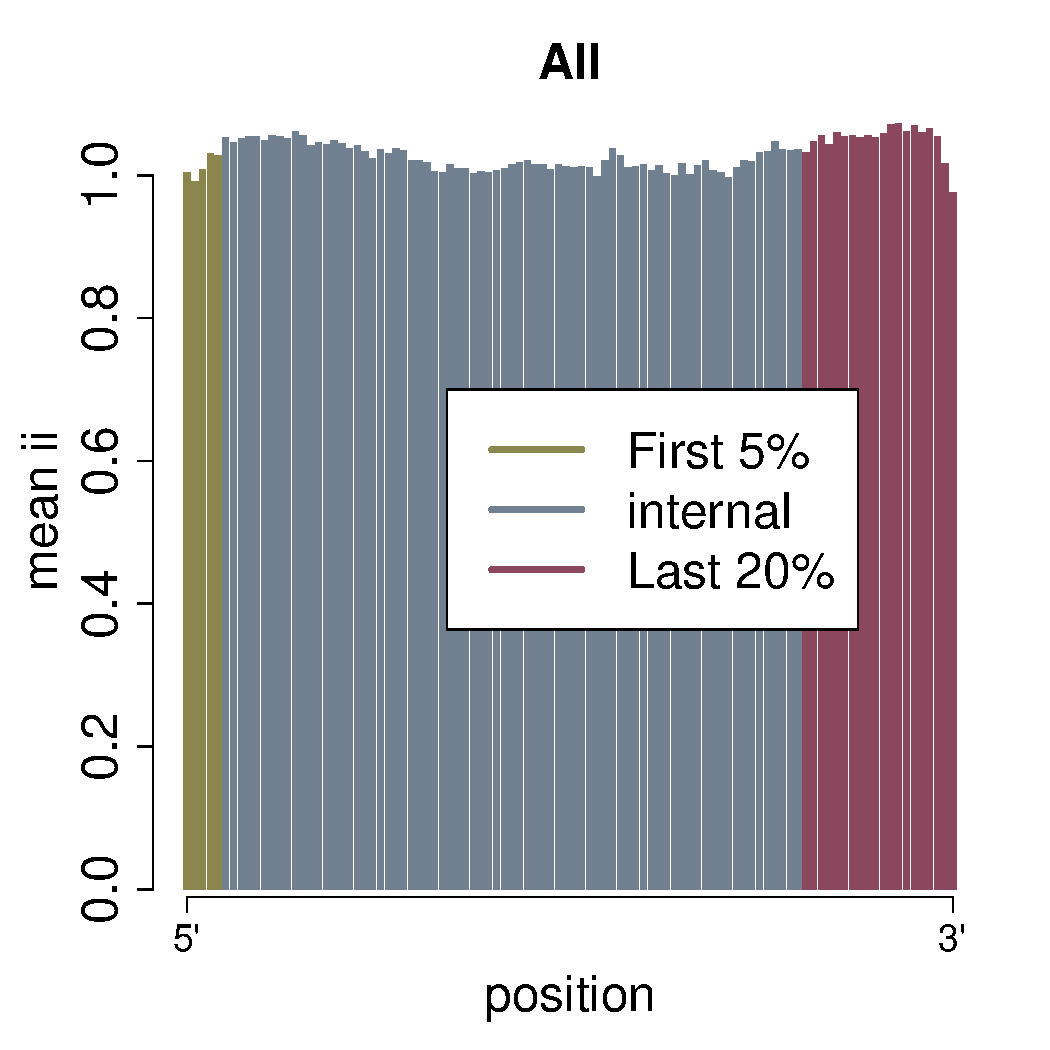
\includegraphics[scale=0.4, page=1]{insertion-position-bias.pdf}&
\includegraphics[scale=0.4, page=2]{insertion-position-bias.pdf}\\
\includegraphics[scale=0.4, page=3]{insertion-position-bias.pdf}&
\includegraphics[scale=0.4, page=4]{insertion-position-bias.pdf}
\end{tabular}
\caption{The plots show the average insertion index in over the genes in all genes (top left), essential genes (top right), non-essential genes (bottom left), and beneficial losses (bottom right). Each bin shows the average insertion index for $1\%$ of the genes. The genes have been divided into 3 segments: 5\% of
the genes on the 5' end, 20\% of the genes on the 3' end, and the rest in the middle. These are shown by khaki, slate gray, and violet red respectively.}
\label{fig:insertion-position-bias}
\end{figure*}

\begin{figure*}
\centering
\begin{tabular}{c c c}
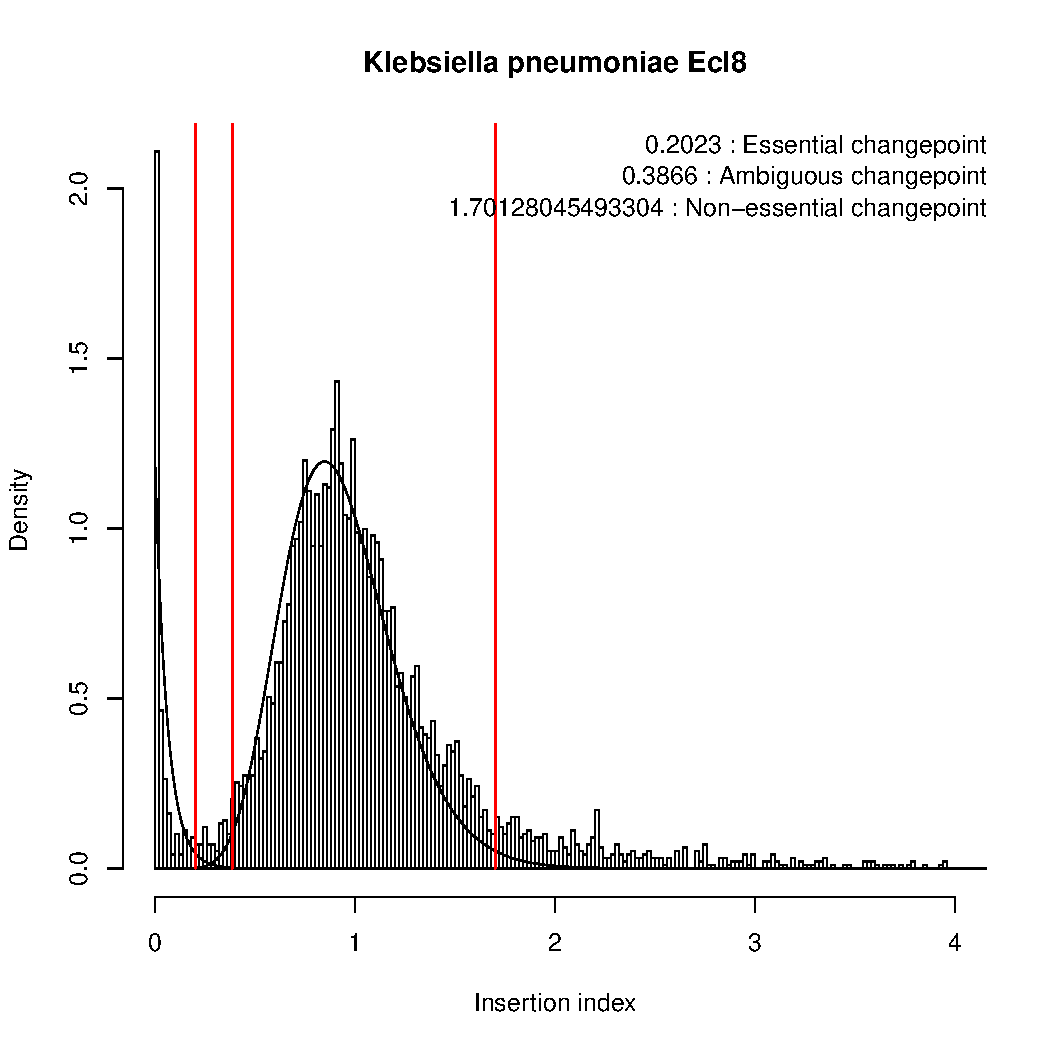
\includegraphics[page=1, scale=0.25]{essentiality-normalised.pdf}&
\includegraphics[page=2, scale=0.25]{essentiality-normalised.pdf}&
\includegraphics[page=3, scale=0.25]{essentiality-normalised.pdf}\\
\includegraphics[page=4, scale=0.25]{essentiality-normalised.pdf}&
\includegraphics[page=5, scale=0.25]{essentiality-normalised.pdf}&
\includegraphics[page=6, scale=0.25]{essentiality-normalised.pdf}\\
\includegraphics[page=7, scale=0.25]{essentiality-normalised.pdf}&
\includegraphics[page=8, scale=0.25]{essentiality-normalised.pdf}&
\includegraphics[page=9, scale=0.25]{essentiality-normalised.pdf}\\
\includegraphics[page=10, scale=0.25]{essentiality-normalised.pdf}&
\includegraphics[page=11, scale=0.25]{essentiality-normalised.pdf}&
\includegraphics[page=12, scale=0.25]{essentiality-normalised.pdf}\\
&\includegraphics[page=13, scale=0.25]{essentiality-normalised.pdf}&\\
\end{tabular}
\caption{Plots show the insertion index distribution for each genome after correcting for distance from the origin of replication bias and bias towards the position of insertion within genes. The plots are divided into 4 regions using red lines. These regions from left to right are: essential, ambiguous, non-essential, and beneficial loss.}
\label{fig:iidist-species-normalised}
\end{figure*}
%\begin{itemize}
%\item There is a bias towards the position of the gene (Fig.~\ref{fig:distance-bias}).
%\item There is a negligible bias towards certain motifs (Fig.~\ref{fig:logos})
%\item The G-C bias needs to be studied further (Fig.~\ref{fig:GC-bias})
%\item The number of insertions on the 3' and 5' ends is more than the internal region in essential genes and less than the internal region in beneficial losses. (Fig.~\ref{fig:insertion-position-bias})
%\end{itemize}
\section{Essentiality and conservation}
To study whether each gene in our 13 organisms is conserved we have proposed a program that clusters homologous proteins. This program uses Jackhmmer from HMMER package~\cite{eddy_accelerated_2011} to compare protein sequences. It first compares a set of query proteins against all given proteins and clusters homologous proteins using Jackhmmer. Then it selects all sequences that were not selected in the first step and compares them together and clusters those protein sequences. In the next step, it breaks down large clusters by using Jackhmmer with more stringent parameters within the clusters and also merges clusters which have a single member by relaxing Jackhmmer parameters. Finally, the program merges overlapping sequences in each cluster and combines similar clusters. The program is summarised in Fig.\@ \ref{fig:homclust} and the distribution of cluster lengths after clustering the genes of 13 strains under study is plotted in Fig.\@ \ref{fig:homclust-results}.

\begin{figure}
\includegraphics[scale=0.2]{homclust.pdf}
\caption{The steps of our proposed algorithm for clustering homologous genes.}
\label{fig:homclust}
\end{figure}

\subsection{Gene classes}
%We needed to cluster sets of orthologous genes in our strains to study the conservation of essentiality. Plenty of methods are proposed for this purpose. Altenhoff et al.\@ have compared 15 of these methods \cite{altenhoff_standardized_2016} and shown that Hieranoid \cite{schreiber_hieranoid:_2013} is among three methods that keep a balance between precision and recall. We have used Hieranoid to cluster the sets of orthologous genes. In addition, we intended to study the essentiality of genes in paralogous genes. For this, we have developed a program that clusters all homologous genes using Jackhmmer from HMMER3 package \cite{mistry_challenges_2013}. 
To study the conservation of genes, we have used homclust and divided the clusters of homologous genes into three groups. Genus specific clusters contain genes that are present only in one genus, the genes in single copy clusters are present in more than one genus and more than 70\% of them are not duplicated, and  the genes in multi-copy clusters are present in more than one genus and less than 70\% of them are not duplicated. These three groups are depicted in Fig.\@ \ref{fig:homclust-results}.

\begin{figure}
\includegraphics[scale=0.3]{cluster-size-dist.pdf}
\caption{Size distribution for all clusters of homologous genes. Genus specific genes are genes that are present only in one genus, single copy genes are present in more than one genus and more than 70\% of them are not duplicated, and multi-copy genes are present in more than one genus and less than 70\% of them are not duplicated.}
\label{fig:homclust-results}
\end{figure}

We have divided the clusters of orthologous genes into 4 groups based on their essentiality (essential, ambiguous, non-essential, and beneficial loss) and 3 groups based on their conservation (genus specific, single copy, and multi-copy). The results are depicted in Fig.\@ \ref{fig:iidist}. The figure shows that most of the essential clusters are single copy and most of the beneficial losses are genus specific.

\begin{figure}
\centering
\includegraphics[scale=0.5]{cluster-essentiality.pdf}
\caption{The genes have been clustered into orthologous groups using Hieranoid and paralogous groups using Jackhmmer and divided into 3 groups: genus specific, single copy, and multi-copy genes. Then, the essentiality of the clusters has been defined using the insertion indices of the genes in the clusters. The figure shows that most of the essential genes are in single copy group, while most of the beneficial losses are genus-specific.}
\label{fig:iidist}
\end{figure}

To study which functions are enriched in each class of essentiality, we have gathered the``note" section for each gene from their embl files. Then, we have counted the repeat number of each word for the genes in each class and the genes that do not belong to that class and the number of all other words in these two groups and used a Fisher's exact test to calculate P-values. The P-values are then corrected using Benjamini-Hochberg-Yekutieli procedure. Fig.\@ \ref{fig:essentiality-pval} shows the top 20 enriched words for each essentiality class. The results show an enrichment of the genes related to replication, transcription, translation, division, and rod shape determining proteins in essential class. The non-essential genes are mostly transport proteins, flagellar proteins, ATPase, and DNA repair proteins. Beneficial losses are enriched in transposase enzymes, putative and hypothetical proteins, and mobile elements. Beneficial losses also contain many fimbrial proteins which probably has occurred because these proteins are not needed in a rich lab medium \textcolor{red}{\{TRUE?\}}.
%We have done a word enrichment analysis on the description of the beneficial losses in Fig.\@ \ref{fig:essentiality-pval}. It shows that most of the beneficial losses are mobile elements. Most of these mobile elements are not included in KEGG database.

We have also conducted a pathway enrichment analysis for these three groups. For this, we have downloaded pathway datasets for strains that were available in KEGG database. This includes pathways for Cirobacter rodentium ICC168, Salmonella Enteritidis P125109, Enterobacter cloacae NCTC 9394, Salmonella Typhimurium D23580, Escherichia coli ETEC H10407, Salmonella Typhimurium SL1344, Escherichia coli K-12 MG1655, and Salmonella Typhi Ty2. Then we have merged these databases and used a hypergeometric test to find which pathways are enriched in each essentiality class. Finally, we have corrected the P-values using Benjamini-Hochberg-Yekutieli. The results are depicted in ~\ref{fig:essentiality-pathway}.

\begin{figure*}
\centering
\begin{tabular}{c c}
\includegraphics[scale=0.4]{essential-pval.pdf}&
\includegraphics[scale=0.4]{non-essential-pval.pdf}\\
\includegraphics[scale=0.4]{beneficialloss-pval.pdf}&
\end{tabular}
\caption{Word enrichment analysis for essential genes, non-essential genes, and beneficial losses compared to other genes. The red line shows P-value = 0.05. The P-values have been calculated using Fisher's exact test and then corrected using Benjamini-Hochberg-Yekutieli procedure.}
\label{fig:essentiality-pval}
\end{figure*}

\begin{figure*}
\centering
\begin{tabular}{c c}
\includegraphics[scale=0.4]{essential-pathways.pdf}&
\includegraphics[scale=0.4]{non-essential-pathways.pdf}\\
\includegraphics[scale=0.4]{beneficialloss-pathways.pdf}&
\end{tabular}
\caption{Pathway enrichment analysis for beneficial losses, essential genes, and non-essential genes compared to other genes. The red line shows P-value = 0.05. The P-values have been calculated using hypergeometric test and then corrected using Benjamini-Hochberg-Yekutieli procedure.}
\label{fig:essentiality-pathway}
\end{figure*}

\subsection{The evolution of essentiality}
%We have compared the number of genes that are conserved in different strains in our study and the number of genes that are essential in these strains. The results propose that although conservation of genes follows a tree-like trend, the essentiality does not show a tree-like signal.
%\begin{itemize}
%\item UpSetR results (Fig.~\ref{fig:upsetr})
%\item Stringent
%\item Dollo law
%\item Ancestral insertion index
%\end{itemize}
%In order to test if the essentiality of genes follows a tree-like trend we have gathered all the genes that are copied once per genome and made a matrix with rows showing genomes and columns showing genes. If a gene is essential in a genome, its corresponding cell in the matrix has value 1 and 0 otherwise. Then we have used the Bray-Curtis distance to generate a distance matrix for the species under study. Finally, a tree has been generated using PHYLIP Neighbor. The resulting tree is not similar to the species tree.
%
%\begin{figure}
%\centering
%\includegraphics[scale=0.2]{neighbor-joining-essentiality-tree.pdf}
%\caption{The tree is generated from all the genes that are copied only once per genome. We have made a binary matrix from the essentiality of these genes. Then, we have generated a distance matrix from these values using Bray-Curtis distance and plotted a phylogenetic tree using PHYLIP Neighbor which uses a neighbour joining method.}
%\label{fig:neighborjoining}
%\end{figure}

In order to test if the essentiality of genes follows a tree-like trend, we have compared the number of genes that are conserved in different strains in our study and the number of genes that are essential in these strains. For this, we have counted the number of genes that are core between every combination of our strains, and the number of genes that are core essential between those combinations. We have used UpSetR package \cite{conway_upsetr:_2016} in R to visualise the results in Fig.\@ \ref{fig:upsetr}. As shown in the figures, among 1908 genes that are core between all the strains under study, only 184 are core essential. The results propose that although conservation of genes follows a tree-like trend (800 genes are core in Klebsiellas, 273 genes are core in Salmonellas, 208 genes are core in Klebsiellas and Enterobacter, ...), the essentiality does not show a tree-like signal and most of the large sets of core essential genes belong to only one strain. We believe this happens due to the small number of essential genes.

\begin{figure*}
\centering
\includegraphics[scale=0.6]{upsetr1-edited.pdf}\\
\includegraphics[scale=0.6]{upsetr2-edited.pdf}
\caption{The first figure shows the number of core genes between each group of species and the second figure shows the number of core essential genes. The bars show the number of genes that are core between the strains marked with black circles. The tick marks show phylogenetically informative columns and the cross marks show non-informative columns.}
\label{fig:upsetr}
\end{figure*}

To test if essential genes are more likely to be conserved, we looked at different levels in the species tree and calculated the ratio of the number of core essential genes to the number of core genes in each level. For the essential genes to be more likely to be conserved, this ratio should increase as we go up in the tree. We have used three different methods for this. The first method is intersecting over core genes and core essential genes, so, genes are core in a node if and only if they are present in all the strains in its child nodes and are core essential if and only if they are essential in all the strains in its child nodes.

The second method which is called ancestral insertion index uses intersection for core genes but a different definition for core essential genes. In this method, we have averaged over the insertion indices of the pair of closest children of the node that we are calculating the core genes for. We have repeated this and averaged the averages until we reached the node under study. Then, we have plotted the insertion indices and fitted an exponential and a gamma distribution to the plot and found the essential genes at that level.

The third method is using Dollo law to define core genes and core essential genes. This method, assumes that the gain of genes (essentiality) is highly improbable, so it tries to have up to one occurrence of gain of genes (essentiality) and minimise the number of times that the genes (the essentiality) has been lost. Using this method, we can predict which genes were present in the common ancestor of our strains and which genes were essential in it. The numbers predicted using these three methods are shown in Fig.\@ \ref{fig:annotated-speciestree}. As this figure shows, the ratio between core essential and core genes is almost constant using the intersection and dollo method; however, this ratio increases as we go higher in the tree using the ancestral insertion index method.

\begin{figure}
\centering
\includegraphics[scale=0.2]{phylosift-aa-raxmlbootstrap-annotated.pdf}
\caption{The tree shows the species tree in Fig.\@\ref{fig:species-tree} annotated by the number of core essential genes and core genes at each node. We have used three methods for defining core essential genes and core genes. The numbers at the leaves are the same using all these three methods. At the internal nodes, red shows the numbers using the intersection method, green shows the ancestral insertion index method, and turquoise shows fdollop method.}
\label{fig:annotated-speciestree}
\end{figure}

As these three methods lead to different results, we have compared the differences between the genes found in these three methods. For this, we have compared the set of core essential genes resulted from intersection and ancestral insertion index methods and performed word enrichment analysis that was explained before on the 184 genes in intersection method and 89 genes that are core essential using ancestral insertion index and not core essential using the intersection method. Moreover, the intersection and fdollop methods and also ancestral insertion index and fdollop method were compared using the same procedure. The results are depicted in Fig.\@\ref{fig:method-difference}.

\begin{figure*}
\centering
\begin{tabular}{c c}
\includegraphics[scale=0.4]{ancestral-intersection-pval.pdf}&
\includegraphics[scale=0.4]{dollo-ancestral-pval.pdf}\\
\includegraphics[scale=0.4]{dollo-intersection-pval.pdf}&
\end{tabular}
\caption{The figure shows the difference between core essential genes in intersection and ancestral insertion index methods, ancestral insertion index and fdollop methods, and intersection and fdollop methods. The red line shows P-value = 0.05. The P-values have been calculated using Fisher's exact test and then corrected using Benjamini-Hochberg-Yekutieli procedure. The top left figure shows words that are enriched in core essential genes found using ancestral insertion index method but not enriched in core essential genes found using intersection method. The top right figure shows words that are enriched in core essential genes found using fdollop method but not enriched in core essential genes found using ancestral insertion index method. The bottom left figure shows words that are enriched in core essential genes found using fdollop method but not enriched in core essential genes found using intersection method.}
\label{fig:method-difference}
\end{figure*}

%\section*{Acknowledgments}
%
%
%\nolinenumbers

%This is where your bibliography is generated. Make sure that your .bib file is actually called library.bib
\bibliography{references}

%This defines the bibliographies style. Search online for a list of available styles.
\bibliographystyle{abbrv}

\end{document}

